\chapter{Rappels théoriques sur les interfaces}
 
Dans ce chapitre nous analysons la dynamique des systèmes statistiques. L'analyse nous permettra de comprendre comment les transitions de phase, notament certains systèmes subissant une séparation de phase à la transition. L'exemple le plus connu est le modèle d'Ising en absence de champ magnétique, ayant la magnétisation comme paramètre d'ordre de la transition. Dans la phase haute température le système est homogène et sa magnétisation est nulle, tandis qu'en dessous de la température critique, dans le cas où le paramètre d'ordre est comservé (par exemple une dynamique de Kawasaki ou modèle B), le système va localement se séparer en deux phases de magnétisation moyenne opposée séparées par une interface minimisant l'énergie de surface entre les deux phases. 
Dans le cas où le paramètre d'ordre n'est pas conservé (par exemple une dynamique de Glauber ou modèle A), une rupture spontannée de symmétrie fera qu'une des deux phases englobe l'autre, au point de recouvrir tout le système (voir Fig \ref{clusterization}). Dans une transition de phase continue où le point critique est atteint depuis l'état désordonné vers l'état ordonné, les domaines de phase égales ont pour taille la longueur de corrélation du système. Dans les transitions de phase telles que celles du modèle d'Ising, la longueur de corrélation diverge lorsque l'on s'approche de la température critique $T_C$. En présence d'un système infini, la longueur de corrélation devient infinie, ce qui implique un que le système prend un temps infini pour atteindre l'équilibre thermodynamique. Ce processus de croissance des domaines depuis s'appelle le \textit{coarsening} et la théorie de la cinétique d'ordre des phases est la théorie qui a été développée pour comprendre le coarsening. 
La thèse s'appuie sur les travaux de cette théorie pour déterminer les propriétés statistiques (telles que la position moyenne et sa tension superficielle) des interfaces entre deux phases coexistantes.

Tandis que l'Hamiltonien d'un système permet d'explorer toutes les configurations d'équilibre possibles, la dynamique du coarsening ne peut être étudiée qu'en construisant un modèle qui explique l'évolution de l'état du système en fonction du temps. Nous verrons tout au long de cette thèse comment la conservation ou non du paramètre d'ordre influe énormément sur la dynamique. Pour de plus complètes informations, se référer à \cite{hohenberg_theory_1977,bray_theory_1994,krapivsky_kinetic_2010,halpin-healy_kinetic_1995}.

Une connaissance parfaite de la fonction de partition nécessite de connaître en tout temps la position de toutes la particules. Les appareils de mesure possèdent tous une résolution spatiale et temporelle, c'est-à-dire qu'ils mesurent l'état moyen de toutes les particules dans un volume et dans un laps de temps donné. Plus la résolution des appareils est bonne, et plus la mesure de la fonction de partition est précise. 
Concrètement, l'appareil de mesure nous donne un champ - par exemple de densité - $\phi(\mx,t)$ de notre système, qui correspond à l'intégration sur un petit volume autour de $\mx$ et une petite durée de temps autour de $x$ de $t$. 

Considérons un système dans l'ensemble canonique d'Hamiltonien  $H(\mq)$ où les $\mq_i$ ($i \in [0,N]$) représentent un nombre fini de degrés de liberté. La fonction de partition est donnée par 
\begin{align}
    Z = \int d\mq e^{-\beta H(\mq)}
\end{align}
avec la probabilité que le système se retrouve dans l'état $\mq$ égale à
\begin{align}
    P_{eq}(\mq) = \frac{e^{-\beta H(\mq)}}{Z}
    \label{eqdis}
\end{align}
À cause du trop grnad nombre de degrés de libertés, la fonction de partition est rarement calculable analytiquement. Dans la limite $\beta \to \infty$ - c'est-à-dire la limite où la probabilité de trouver la configuration du système minimisant le plus l'énergie - l'intégrale peut s'approcher par la méthode de Laplace pour l'évaluation des intégrales 
\begin{align}
    Z_{MF}= e^{-\beta H(\mq^*)}
\end{align}
Le champ $\mq^*$ est le champ qui minimise $H$ dont les degrés de liberté sont déterminés par
\begin{align}
    \frac{\partial H}{\partial q_i}|_{\mq={\bf q^*}}=0.
\end{align}
Ce champ $\mq^*$ est le \textbf{champ moyen}, puisqu'il est le champ le plus probable. Dans cette approximation de champ moyen, toute observable est donnée par
\begin{align}
    < f(\mq) > = f(\mq^*)
\end{align}

We now consider how one can model dynamics of such systems. We will look for a Langevin equation which is chosen to give the correct equilibrium Gibbs-Boltzmann distribution. We write
\begin{align}
\frac{d q_i}{dt} = -L_{ij}\frac{\partial H(\mq)}{ \partial q_j} + \eta_i(t),
\end{align}
where $L_{ij}$ is a matrix which discuss later and $\eta_i(t)$ is zero mean Gaussian white noise  with correlation function 
\begin{align}
\langle \eta_i(t)\eta_j(t')\rangle =  \Gamma_{ij} \delta(t-t'),\label{cfn}
\end{align}
The Gaussian white noise represents the effects of thermal fluctuations on the system we assume that the correlation time of these fluctuations is extremely short with respect to the dynamics of the degrees of freedom $q_i$ (in fact in critical systems the dynamics becomes very slow, critical slowing down, and this approximation becomes better and better as one approaches the critical point).  As Eq. (\ref{cfn}) is for a correlation function the matrix $\Gamma_{ij}$ must be symmetric and cannot have any negative eigenvalues.

In the absence of noise or thermal fluctuations, so at zero temperature, the system will simply minimise its energy. Therefore if 
\begin{align}
\frac{\partial H(\mq)}{ \partial q_j} =0, 
\end{align}
with no noise we have $\frac{d q_i}{dt}=0$, that is to say it is the term $\frac{\partial H(\mq)}{ \partial q_j}$ that drives the dynamics if there is no noise. As long as the matrix $L_{ij}^{-1}$ exists the zero temperature dynamics will take the system to the local minimum of $H$ and to the absolute minimum if there are no metastable configurations. 

Under these assumptions, the Fokker-Planck equation for the probability density function of the degrees of freedom is 
\begin{align}
\frac{\partial p(\mq,t)}{\partial t} = \frac{\partial}{\partial q_i} \left[\frac{1}{2}\Gamma_{ij} \frac{\partial p(\mq,t)}{\partial q_i} + p(\mq,t) L_{ij}\frac{\partial H(\mq)}{ \partial q_j}\right].
\end{align}
This can be written as 
\begin{align}
\frac{\partial p(\mq,t)}{\partial t} +\frac{\partial}{\partial q_i}J_i(\mq,t)=0,
\end{align}
where the ${\bf J}(\mq,t)$ is the probability current. We now insist that the system is in equilibrium with zero current when $p(\mq,t)= P_{eq}(\mq)$ as given by Eq. (\ref{eqdis}), this gives
\begin{align}
\left[-\frac{\beta}{2}\Gamma_{ij} + L_{ij}\right]\frac{\partial H(\mq)}{ \partial q_j},
\end{align}
and this holds for any choice of $H$ is we chose.
\begin{align}
\Gamma_{ij}= 2T L_{ij}
\end{align}
where we have taken units where Boltzmann's constant $k_B=1$. 
\section{Statistical field theory}
We now consider a system with Hamiltonian $H[\phi]$ which depends on a continuous field 
$\phi({\bf x})$. The partition function is given by a functional integral
\begin{align}
Z = \int d[\phi] \exp(-\beta H[\phi]),
\end{align}
the functional integral over all possible fields $\phi$ can be taken as a limit where $\phi$ is defined at a finite number of points on a lattice and then the lattice spacing is taken to zero. 

The mean field approximation to partition function is then given by
\begin{align}
Z _{MF}=  \exp(-\beta H[\phi_{MF}]),
\end{align} 
where $\phi_{MF}$ is the mean field solution which minimises $H$. The definition of a functional derivative of a functional 
\begin{align}
F[\phi+\delta\phi]-F[\phi]= \int d{\bf x} \frac{\delta F}{\delta\phi({\bf x})} \delta\phi({\bf x}).
\end{align}
Therefore if a field $\phi$ maximises $H$ we must have 
\begin{align}
\frac{\delta H}{\delta\phi({\bf x})}=0.
\end{align}

We now consider the standard Landau-Ginzburg Hamiltonian describing Ising like systems where
\begin{align}
H[\phi] = \int d{\bf x} \ \frac{\kappa}{2}[\nabla \phi]^2 + V(\phi) .
\end{align}
The first term represents an energetic cost of varying the field $\phi$ while the second potential term has two minima at $\phi=\pm \phi_c$, and without loss of generality we can chose  $V(\phi_c)=V(-\phi_c)$, in the low temperature or phase separated phase and a single minimum at $\phi=0$ in the high temperature phase. The standard, so called, $\phi^4$ form is
\begin{align}
V(\phi) = \frac{1}{2} m^2 \phi^2 + \frac{\lambda}{4!} \phi^4,\label{p4}
\end{align} 
where 
\begin{align}
m^2 = T-T_c.
\end{align}
It is easy to see that 
\begin{align}
\frac{\delta H}{\delta \phi({\bf x})} = -\kappa \nabla^2 \phi({\bf x}) + V'(\phi).\label{cm}
\end{align}
If there is non constraint on the system if can simply chose $\phi({\bf x}) =\phi_c$ or $\phi({\bf x}) =-\phi_c$ everywhere which corresponds to a  free energy $F=H[\phi_c]=0$. However in a system with a conserved order parameter
\begin{align}
\int d{\bf x} \  \phi({\bf x})=0, 
\end{align}
then the solutions $\phi=\pm \phi_c$ cannot hold. In this case the system will separate into a two phases where $\phi({\bf x})= \pm \phi_c$. We therefore choose an interface at $z=0$ where 
and take $\phi({\bf x}) = \phi_K(z)$ ($K$ standing for kink as it is known as the kink solution in the literature) where $\lim_{z\to\-\infty}=-\phi_c$ and  $\lim_{z\to\infty}=-\phi_c$. 
We therefore find from Eq. (\ref{cm}) that
\begin{align}
-\kappa \frac{d^2 }{dz^2}\phi_K(z)  + V'(\phi_K) = 0 \label{kk0}
\end{align}
This equation can be solved for the potential in Eq. (\ref{p4}) ({\em you should do it and fill in the details}) but even without knowing the explicit solution we can write
\begin{align}
H[\phi_K]=  A\int dz \ \frac{\kappa}{2}\left(\frac{d\phi_K(z)}{dz}\right)^2 + V(\phi_K(z)),\label{kk1}
\end{align}
where $A$ is the surface area of the system in the plane perpendicular to the direction $z$. 
However if we multiply Eq. (\ref{kk0}) by $d\phi/dz$ and integrate we find
\begin{align}
-\frac{\kappa}{2} (\frac{d\phi_K}{dz})^2 + V(\phi) = C,
\end{align}
where $C$ is a constant. However as $\phi_K(z)\to \pm \phi_c$ as $z\to \pm \infty$ and $V(\pm\phi_c) =0$ we find that $C=0$. Using this we obtain 
\begin{align}
H[\phi_K]=  A\int dz\  {\kappa}\left(\frac{d\phi_K(z)}{dz}\right)^2 .
\end{align}
If the interface has a free energy per unit area of $\sigma$ then we have the Cahn-Hillard estimate of the surface tension 
\begin{align}
\sigma=  \int dz\  {\kappa}\left(\frac{d\phi_K(z)}{dz}\right)^2 .
\end{align}

Now we return to dynamics. If we compare with systems with a discrete number of variables we
should have a Langevin equation of the form
\begin{align}
\frac{\partial \phi({\bf x})}{\partial t}= -L \frac{\delta H}{\delta \phi({\bf x})} + \eta({\bf x},t).
\end{align}
The white noise correlator should have the form
\begin{align}
\langle \eta({\bf x},t)\eta({\bf x}',t)\rangle =\delta(t-t')\Gamma({\bf x},{\bf x'}),
\end{align}
where here  $\Gamma({\bf x},{\bf x'})$ is an operator (before it was a matrix) defined by its action on functions $f$ as
\begin{align}
\Gamma f({\bf x}) = \int d{\bf x}' \Gamma({\bf x},{\bf x}')f({\bf x}'),
\end{align}
and $L$ is also an operator with 
\begin{align}
L f({\bf x}) = \int d{\bf x}' L({\bf x},{\bf x}')f({\bf x}'),
\end{align}
Following the same arguments for systems with a finite number of degrees of freedom we thus have the relation
\begin{align} 
\Gamma({\bf x},{\bf x}') =2T L({\bf x},{\bf x}').
\end{align}
The simplest form of dynamics is given by $L({\bf x},{\bf x}')=\alpha\delta({\bf x}-{\bf x}')$ which gives the model A dynamics
\begin{align}
\frac{\partial \phi({\bf x})}{\partial t}= -\alpha \frac{\delta H}{\delta \phi({\bf x})} + \eta({\bf x},t),
\end{align}
with the noise correlator
\begin{align}
\langle \eta({\bf x},t)\eta({\bf x}',t)\rangle =2T \alpha \delta(t-t')\delta({\bf x}-{\bf x'}).
\end{align}
The average value of $\phi$ 
\begin{align}
\overline \phi(t) = \frac{1}{V}\int d{\bf x} \phi({\bf x},t),
\end{align}
is clearly not generally conserved by this dynamics.

Model $B$ dynamics amounts to choosing
\begin{align}
L({\bf x}-{\bf x}')= -D\nabla^2 \delta({\bf x}-{\bf x'}),
\end{align}
here the fact that $L$ is a positive semi-definite operator can be seen by taking its Fourier transform. The evolution equation here is
\begin{align}
\frac{\partial \phi({\bf x})}{\partial t}= D\nabla^2 \frac{\delta H}{\delta \phi({\bf x})} + \eta({\bf x},t),
\label{MB}
\end{align}
and where
\begin{align}
\langle \eta({\bf x},t)\eta({\bf x}',t)\rangle =-2TD   \delta(t-t')\nabla^2\delta({\bf x}-{\bf x'}).
\end{align}
We notice that if we introduce the vectorial white noise with components $\eta_i({\bf x},t)$ such that
\begin{align}
\langle \eta_i({\bf x},t) \eta_i({\bf x}',t')\rangle =\delta_{ij} \delta({\bf x}-{\bf x'})\delta(t-t),
\end{align}
where $\delta_{ij}=1$ for $i=j$ and is zero otherwise,  we can write
\begin{align}
\eta({\bf x},t)= \nabla\cdot {\boldsymbol \eta}({\bf x},t),
\end{align}
as one can verify the two noises have the same correlation function. In this way Eq. (\ref{MB}) becomes 
\begin{align}
\frac{\partial \phi({\bf x})}{\partial t}= \nabla\cdot[ D\nabla \frac{\delta H}{\delta \phi({\bf x})} + {\boldsymbol\eta}({\bf x},t)].
\end{align}
From this it is easy to see that the order parameter is conserved - thus model  B describes conserved phase ordering dynamics.

The above argument is rather phenomenological and a microscopic derivation of conserved order parameter dynamics gives the so called Dean-Kawasaki equation. Model B is a simplified form of this exact equation - you could say more.



Prenons un système composé de deux types de particules A et B qui se repoussent mutuellement, comme un ensemble liquide/gaz ou un fluide binaire du genre vinaigrette. À chaque point de l'espace $x$ on peut associer la présence de la particule la plus proche par la fonction $n(x,t) = A \text{ ou } B$. Ici, les particules sont supposées indiscernables entre elles. Dans le cas où les particules seraient discernables, ce qui n'est jamais le cas dans les expériences mais l'est dans les simulations numériques, il est plus correct d'invertir la fonction par $n_i(t) = x$, où $i$ est le label de chaque particule, qu'elle soit de type A ou B. 
Il est plus convenable que la fonction $n(x,t)$ donne un nombre plutôt qu'un type de particules. Nous supposons que les deux types de particules $A$ et $B$ se comportent comme des pôles électriques de signe opposés, puisque qu'elles s'attirent entre particules du même type mais se repoussent si elles ne le sont pas. Le module de la force d'interaction entre particules peut toujours être factorisée en dehors de la fonction de partition, si bien que l'on peut poser que
\begin{align}
    n(x,t) = \begin{cases} -1 &\text{ si particule A} \\ 1 &\text{ si particule B}  \end{cases}
\end{align}
Une fois définie cette fonction, un paramètre d'ordre convenable est la magnétisation totale du système
\begin{align}
    m(t) = <n(x,t)>_x = \frac{1}{V} \int d^dx  n(x,t)
\end{align}
Les particules ont la possibilité de réagir par la réaction chimique $A \leftrightarrow B$ dans un système chimique, par inversion de spin dans un système ferromagnétique, ou par échange avec un réservoir si l'échelle de temps de l'échange est bien inférieure à l'échelle de temps du système. Dans tous ces cas, le paramètre d'ordre $m(t)$ n'est pas conservé et, si nous sommes à l'équilibre thermodynamique, fluctue autour d'une valeur moyenne $m$.  Dans la classification de Hohenberg et Halperin\cite{hohenberg_theory_1977}, ces systèmes appartiennent au \textbf{modèle A}, qui décrit les systèmes dans l'ensemble grand-canonique.

Les particules peuvent également diffuser par échange de place entre deux particules voisines, et aucune particule ne peut être créée ou détruite. Le paramètre d'ordre est maintenant conservé dans le temps. Il est possible d'imposer, via les conditions initiales, un paramètre d'ordre à l'équilibre thermodynamique canonique différent de celui que l'on aurait dans l'ensemble grand-canonique. Ces systèmes sont décrits par le \textbf{modèle B}.

Dans ce chapitre, nous introduisons les principaux résultats de la physique des interfaces dans chaque ensemble thermodynamique, ainsi que les principales méthodes d'analyse. 

    \section{Théorie de champ moyen}

Une connaissance parfaite de la fonction de partition nécessite de connaître en tout temps la position de toutes la particules. Les appareils de mesure possèdent tous une résolution spatiale et temporelle, c'est-à-dire qu'ils mesurent l'état moyen de toutes les particules dans un volume et dans un laps de temps donné. Plus la résolution des appareils est bonne, et plus la mesure de la fonction de partition est précise. 
Concrètement, l'appareil de mesure nous donne un champ moyen $\phi(x,t)$ de notre système, qui correspond à l'intégration sur un petit volume autour de $x$ et une petite durée de temps autour de $t$ de $n(x,t)$. 
Puisque ce champ moyen représente une densité, de particules $A$ et $B$ de valeur $-1$ et $+1$ respectivement, la fonction $\phi$ a pour valeurs dans $[-1,1]$.
Par exemple, on peut dire que si à un endroit et à un temps donné, il n'y que des particules de type A, $\phi(x,t)=-1$, tandis que $\phi(r,t)=+1$ pour les particules B. Le paramètre d'ordre est maintenant donné par
\begin{align}
    m(t) = <\phi(x,t)>_x = \int d^dx  \phi(x,t)
\end{align}

\begin{figure}[h]
    \centering
    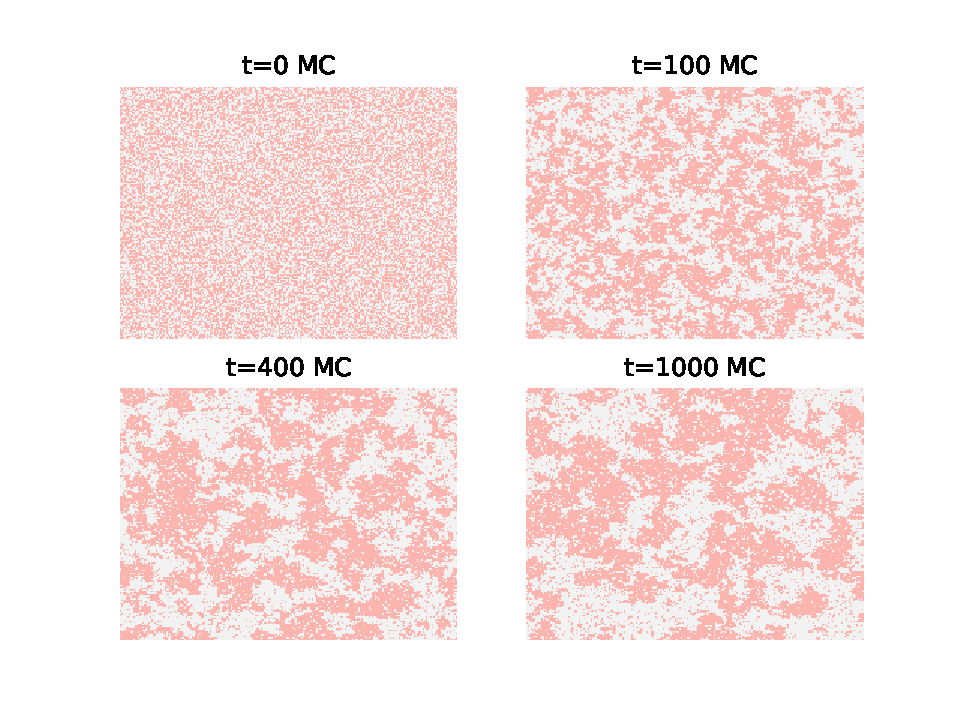
\includegraphics[width=0.9\linewidth]{intro/clusterization.pdf}
    \caption{Phénomène d'aggrégation à partir d'un refroidissement (\textit{quench}) dans un modèle d'Ising de $T=\infty$ à $T=T_C$ pour différents temps en étapes de Monte Carlo, pour un système $600 \times 600$ avec une dynamique non-conservée de Glauber.}
    \label{clusterization}
\end{figure}

À température non nulle, les fluctuations thermiques vont créer un système non-uniforme possédant des clusters possédant une longueur de corrélation $\xi$. L'énergie d'interaction de ces clusters est donné par l'Hamiltonien de Ginzburg-Landau\cite[§ 45]{l_landau_physique_1990}
\begin{align}
    H_0 &= \int d^dx \frac{\kappa}{2}(\nabla \phi)^2 + V(\phi) =  \int d^dx \frac{\sigma}{2}(\nabla \phi)^2 + \frac{\lambda}{2}(\phi^2-1)^2
    \label{hamil-mean-field}
\end{align}
où le premier terme correspond à la tension superficielle cherchant à diminuer les variations au sein du système, et le second terme est un potentiel en double puit $V(\phi) = \frac{\lambda}{2}(\phi^2-1)^2$ \ref{double-puits} simulant une interaction repoussante entre les deux types de particules. Ce terme explique la création de clusters de la figure \ref{clusterization}.

Dans les expériences en laboratoire, les systèmes sont souvent couplés à des champs magnétiques ou chimiques $h(x)$ d'Hamiltonien
\begin{align}
    H_1 &= - \int d^dx h(x)\phi(x)
    \label{champ-externe}
\end{align}
qui induit un changement de stabilité entre les phases, le signe négatif étant pour que le système s'aligne sur le champ. 
\begin{figure}
    \centering
    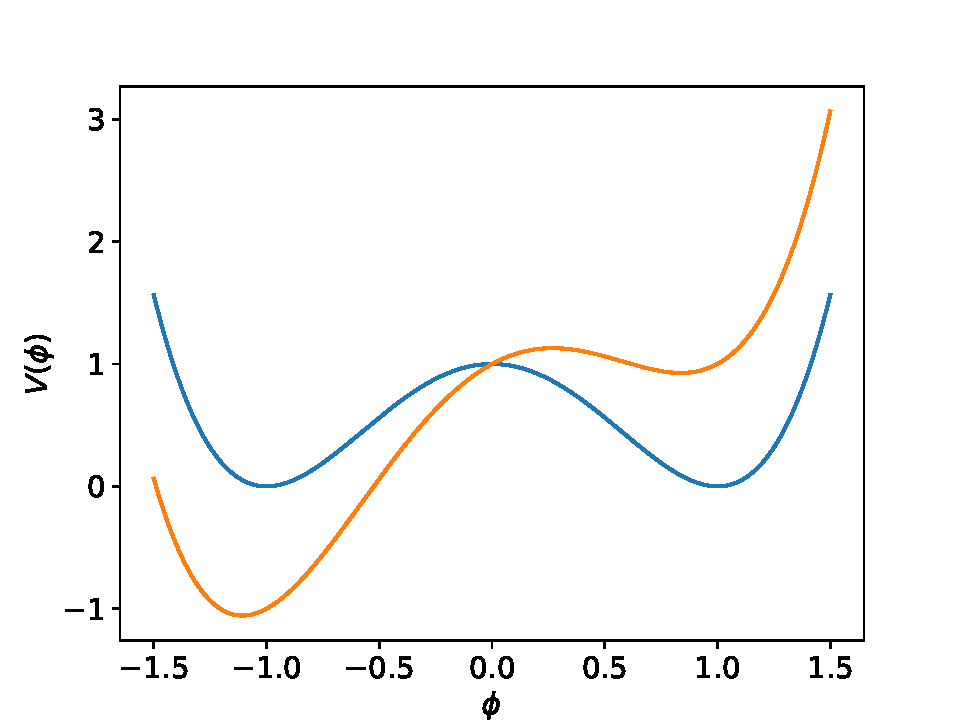
\includegraphics[width=0.5\linewidth]{intro/shift.pdf}
    \label{double-puits}
    \caption{Potentiel en double puits \ref{hamil-mean-field} pour $\lambda = 1$ en bleu. Le potentiel a deux positions d'équilibre stables à $\pm1$, ce qui induit une séparation de phase. En orange, l'ajout d'un champ externe \ref{champ-externe} constant $h \phi(x)$ rend la phase $+1$ métastable.}
\end{figure}

La fonction de partition du système s'écrit
\begin{align}
    \mZ = \int D[\phi] e^{-\beta( H)}
\end{align}
avec $H= H_0 + H_1$. Dans le cas où le paramètre d'ordre est conservé avec pour valeur fixe $M$, un terme supplémentaire égal à $\delta(\int d^dx \phi(x)-M)$ apparaît. Ce terme empêche toute résolution analytique de la fonction de partition, mais nous verrons plus tard certaines méthodes pour contourner ce problème.
La valeur moyenne de $\phi$ est alors
\begin{align}
    <\phi> = - \frac{\delta F}{\delta h(x)}
\end{align}
qui est nul en l'absence d'un champ extérieur $h(x)$. La fonction de corrélation à deux points de cet Hamiltonien est donné par 
\begin{align}
    C(x,y) = <\phi(x)\phi(y)> =  \frac{k_B T}{\sigma} \int_q \frac{e^{iq(x-y)}}{\xi^{-2}+ q^2}
\end{align}
et le facteur de structure  par
\begin{align}
    S(k) = < \tilde{\phi}(k)\tilde{\phi}(q)> = (2\pi)^d \delta_{k,q} \frac{k_B T}{\sigma} \frac{1}{\xi^{-2}+ q^2}
\end{align}
où l'on voit apparaître ici la longueur de corrélation à l'équilibre $\xi$. 

Dans l'ensemble grand-canonique, les particules ont la possibilité de se transformer en d'autres particules par réaction chimique ou par exemple inversion des spins dans un système ferromagnétique. L'équation dépendante du temps de Ginzburg-Landau (TDGL) décrit l'évolution du champ moyen en minimisant l'énergie libre du système
\begin{align}
    \frac{\partial \phi}{\partial t} &= - \alpha \frac{\delta H}{\delta \phi} \\
    &= \frac{\delta H}{\delta h} \frac{\delta h}{\delta \phi}
    \label{tdgl}
\end{align}
Le terme $\alpha$ est un coefficient cinétique décrivant le temps de relaxation du système. La minimisation de l'énergie tend à minimiser l'interface entre les différentes phases ainsi qu'à privilégier les phases homogènes. Dans un système infini, afin de minimiser la tension superficielle, les clusters grandissent au fur et à mesure de sorte que la longueur de corrélation $\xi$, qui décrit la longueur typique des phases, augmente comme $\xi(t) \propto t^{1/2}$.

Ces clusters sont définis pas l'interface\footnote{Dans les systèmes 1D, on retrouve le terme de mur entre deux domaines (\textit{domain wall}).} comme une courbe imaginaire où nous avons, en moyenne, un très fort gradient du champ $\phi$. 
En considérant que de part et d'autre du système nous avons deux phases différentes complètement homogènes selon l'axe des $z$, c'est-à-dire $\phi(z \to -\infty) = -1$ et $\phi(z \to +\infty) = +1$, on peut minimiser l'énergie libre selon $z$ afin d'obtenir le profil de l'interface. L'équation $\frac{\delta H}{\delta \phi} = 0$ nous donne une équation différentielle du second ordre en $\phi$ qui a pour solution selon l'axe $z$
\begin{align}
    \phi(z) = \tanh(\frac{1}{\xi_\perp} (z-h))
    \label{profil-phi}
\end{align}
où $\phi(z)$ est moyennée sur les autres variables spatiales et sur le temps, $\xi_\perp = (2\lambda)^{-\frac{1}{2}}$ est la largeur moyenne de l'interface, et $h$ est la hauteur moyenne de l'interface, que l'on peut fixer comme on le désire. Bien sûr, cette équation n'est valable qu'à la frontière entre deux domaines. Proche d'une transition de phase, la longueur de corrélation de l'interface $\xi_\perp$  diverge selon des exposants critiques spécifiques à chaque classe d'universalité. Pour une étude complète des exposants critiques pour chaque classe d'universalité, se référer à \cite{pelissetto_critical_2002}. 

{\color{red} réécrire}
La tension superficielle est donnée par l'énergie apportée par l'interface comparée à un milieu parfaitement homogène, c'est-à-dire où le terme $\frac{1}{2}(\nabla \phi)^2$ de l'hamiltonien est nul. La densité d'énergie par unité de surface est donc
\begin{align}
    \sigma = H_{inhomogène} - H_{homogène} = \int_{-\infty}^\infty dz \left(\frac{\partial \phi}{\partial z} \right)^2
\end{align}

Dans le \textbf{modèle B}, c'est-à-dire dans l'ensemble canonique, les particules ne peuvent réagir chimiquement entre elles. Avec l'agitation thermique, les particules auront cependant tendance à se déplacer, en échangeant leur position avec celle de leur plus proche voisin. Cette dynamique locale, qui décrit les phénomènes locaux comme la diffusion, est régie par l'équation de Cahn-Hillard\cite{cahn_free_nodate,langer_new_1975,kawasaki_growth_1978}
\begin{align}
    \frac{\partial \phi}{\partial t} = D \nabla^2 \frac{\delta H}{\delta \phi} 
    \label{cahn-hillard}
\end{align}
où $D$ est la diffusivité des particules. Dans cette dynamique plus lente, la taille typique des clusters est de l'ordre de $\xi(t) \propto t^{1/3}$.

\begin{figure}
    \centering
    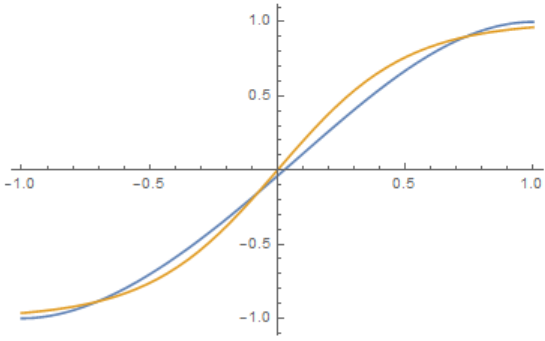
\includegraphics[width=0.5\linewidth]{intro/profil-KawVsGlau.png}
    \caption{Profil de l'interface pour un paramètre d'ordre conservé (orange) et non-conservé (bleu) avec les conditions aux limites $\phi(+\infty)-1$ et $\phi(+\infty)=+1$. Pour le modèle non-conservé, la résolution de l'équation \label{langevin-kawasaki} nécessite deux autres conditions supplémentaires. Nous avons donc mis $\phi(-1)=-1$,$\phi(1)=1$,$\phi'(-1)=\phi'(1)=0$. {\color{red} relancer code en résolvant la solution conservée au lieu de tanh(2x). Besoin mathematica.}}
\end{figure}

L'ajout d'un terme de bruit thermique aux équations de Langevin \ref{tdgl} et \ref{cahn-hillard} leur donne une la même allure que les modèles \textbf{A} et \textbf{B} respectivement de la théorie de la dynamique au point critique\cite{hohenberg_theory_1977}. Les équations précédents sont bien une approximation à $T=0$.


    \section{Taille finie et effet Casimir critique}
    
Sans perte de généralités en 3D, supposons un système de taille $L\times L' $ où $L<L'$. L'énergie libre $F(\beta,L,L') = - \frac{1}{\beta} \ln ( Z(\beta,L,L'))$ est une grandeur extensive lorsque la longueur de corrélation est plus petite que la taille du système $L$. 
Cette énergie libre peut se décomposer entre l'énergie de chaque phase $\omega_{bulk}$ et l'énergie de tension superficielle aux interfaces $\omega_{surf}$ \cite[§4]{cardozo_finite_2015}. À noter qu'à haute température dans un système complètement homogène, ce dernier terme disparaît.

Cependant, lorsque $\xi \simeq L$, la contrainte exercée sur les fluctuations thermiques par les conditions aux bords implique une modification de l'énergie libre, créant une force les parois. Cet effet, premièrement prédit Hendrik Casimir\cite{h_b_g_casimir_attraction_1948}, fut étendu aux systèmes critiques\cite{nikolic_is_2017}, où la divergence de la longueur de corrélation rend les expériences bien plus faciles\cite{nguyen_controlling_2013}.

L'énergie libre d'un tel système se décompose maintenant en 
\begin{align}
    \Omega(\beta,L,L') = L \omega_{bulk}(\beta) + \omega_{surf}(\beta) + L \omega_{ex}(\beta,L)
    \label{decomposition-energie}
\end{align}
où $\omega_{bulk}(L)$ est le surplus d'énergie libre due au confinement des fluctuations, qui devient nul dans la limite $L\to \infty$.

La force de confinement est définit par 
\begin{align}
    F_\perp(\beta,L) = - \frac{1}{L' }\frac{\partial \Omega}{\partial L} \bigg|_{\beta,L'} = -  \omega_{bulk}(\beta) -  \frac{\partial \omega_{ex}(\beta,L)}{\partial L}\bigg|_{\beta,L'}
\end{align}
où le premier terme est la pression exercée par le système, tandis que le second terme est la force de Casimir, qui n'est pas extensive. Afin d'extraire la force de Casimir, il suffit alors de soustraire deux quantités extensives, c'est-à-dire 
\begin{align}
    F_\perp(\beta,L_1) - F_\perp(\beta,L_2) =   \frac{\partial \omega_{ex}(\beta,L_2)}{\partial L_2}\bigg|_{\beta,L'} -  \frac{\partial \omega_{ex}(\beta,L_1)}{\partial L_1}\bigg|_{\beta,L'}
\end{align}
Puisque le surplus d'énergie est nul lorsque $L\to \infty$, on obtient que
\begin{align}
    F_\perp(\beta,L_1) - F_\perp(\beta,\infty) =   -  \frac{\partial \omega_{ex}(\beta,L_1)}{\partial L_1}\bigg|_{\beta,L'}
\end{align}
Cardozo et Holdsworth\cite[§5]{cardozo_finite_2015} ont développé une méthode numérique de calcul pour calculer numériquement cet excès. Nous y reviendrons plus tard.




    \section{Modèles d'interface}

Dans la réalité, les phases sont extrêmement inhomogènes, avec des bulles ou des digitations qui empêchent une description dynamique aisée de l'interface. Si l'on désire étudier l'interface de ces bulles ou digitations, où localement l'interface est bien définie par une fonction d'une seule variable, l'approche du champ moyen suffit. C'est le cas par exemple des régimes d'échelle (\textit{scaling regime}) où les interfaces se comportent toujours de façon correcte. De la même manière, ce régime d'échelle peut s'obtenir dans un milieu inhomogène en supposant qui'il est, au contraire, homogène. On suppose dans ce cas qu'il n'y a ni digitation ni bulles d'évaporation. Dans cette approximation l'interface est parfaitement définie en un point $h(x)$ (et non dans un profil comme dans \ref{profil-phi}. Tous les points du champ se trouvant en bas de l'interface prennent une unique valeur strictement différente de tous les points du champ au-dessus de l'interface. Sans perte de généralité, nous pouvons séparer les variables spatiales par $x$ pour toutes les coordonnées parallèles à l'interface et par $z$ la coordonnée transverse. Cela se traduit par
\begin{align}
    \phi(z) = f(z-h(x))
    \label{capillary-wave-theory}
\end{align}
où $f(x\greater 0) = \phi_1$ et $f(x\less 0) = \phi_2$. Notre système est maintenant complètement défini par l'interface $h(x)$ d'Hamiltonien
\begin{align}
    H = \int d^d x \frac{\sigma}{2} (\nabla h(x))^2 + V(h)
    \label{hamil-cwt}
\end{align}
où le premier terme est l'analogue au premier terme dans \ref{hamil-mean-field} représentant la tension superficielle et le potentiel $V$ fait référence au champ externe \ref{champ-externe}. 
Une interface se caractérise le plus généralement sa hauteur moyenne $<h(t)>$ de l'interface dans l'espace, et sa fonction de corrélation parallèle à l'interface qui décrit les modes de fluctuation de l'interface (sa rugosité)
\begin{align}
    C_\parallel(r,t) = <h(x,t)h(x+r,t)>_x - <h(0,t)>^2 = \sum_i A_i(\frac{r}{\xi_i}) 
\end{align}
Comme démontré dans la section \ref{sec_laser}, la décroissance spatiale est une somme de modes $i$ ayant des longueurs de corrélation différentes $\xi_i$ à décroissance exponentielle dont, dans la limite thermodynamique, seul le mode de plus basse énergie est observable. 
L'épaisseur de l'interface est donnée par $\omega(t) = \sqrt{C_\parallel(0,t)} = \sqrt{<h(t)^2> - <h(t)>^2}$. Cet observable est très facilement calculable dans les simulations de Monte Carlo.


    \subsection{Paramètre d'ordre non conservé}

Supposons une surface à laquelle viennent s'agréger des particules provenant d'un réservoir afin de créer un dépot. L'interface est alors définie par la hauteur de l'aggrégat par rapport à la surface de dépôt.

En partant de \ref{tdgl} et en insérant \ref{capillary-wave-theory} avec le changement de variable $u= z-h$, on a \cite{bray_interface_2001}
\begin{align}
    \frac{\partial h}{\partial t} f'(u) &= \nabla^2 h f'(u) - V'(f) + \xi(x,t)
\end{align}
avec $\xi(x,t)$ un bruit blanc gaussien. En multipliant les deux côtés par $f'(u)$ et en intégrant de $-\infty$ à $+\infty$, puisque le terme $ \int_{-\infty}^\infty V'(f) f'(u) du = 0$, on obtient l'équation d'Edwards-Wilkinson \cite{edwards_surface_1982} 
\begin{align}
     \frac{\partial h}{\partial t} = D + D \nabla^2 h +  \eta(x,t)
    \label{edwards-wilkinson}
\end{align}
où $\eta(x,t)$ est un bruit blanc de moyenne nulle et de corrélation 
\begin{align}
    <\eta(x,t)\eta(x',t')> = 2 D T\delta(x-x')\delta(t-t')
\end{align}
Ici $D+ \sqrt{2 D T} \eta(x,t)$ est le flux de particules s'aggrégeant en fonction du temps et $D \nabla^2 h$ dépend de la forme de l'interface, favorisant ou non le dépôt de particules à certains endroits.
La hauteur moyenne de l'interface varie donc comme $<h(t)> = Dt$. En se positionant dans le référentiel de l'interface via la transformation $h \rightarrow h + Dt$, on obtient
\begin{align}
     \frac{\partial h}{\partial t} =   \nabla^2 h +   \eta(x,t)
    \label{edwards-wilkinson-conesrved}
\end{align}
On remarquera la similarité entre cette équation et l'équation \ref{tdgl} en l'absence de potentiel en double puits et de champ externe.

L'ajoute d'un potentiel en double puits est cependant nécessaire afin d'obtenir une séparation de phases. L'équation KPZ\cite{kardar_dynamic_1986} étudie un champ moyen en $\phi^4$, ce qui introduit des nonlinéarités indispensables pour certaines propriétés des interfaces.
\begin{align}
     \frac{\partial h}{\partial t} = D \nabla^2 h +  \lambda (\nabla h)^2 + \eta(x,t)
    \label{kpz}
\end{align}

Il est intéressant de calculer la probabilité de distribution de la hauteur de l'interface par rapport à sa moyenne. La probabilité $p(h$) de trouver l'interface à la distande $h$ de la hauteur moyenne est donnée par l'équation de Focker-Planck\cite[p.241]{halpin-healy_kinetic_1995} associée à \ref{edwards-wilkinson-conesrved}
\begin{align}
    \frac{\partial p(h,t)}{\partial t} = - \int dx \frac{\delta}{\delta h} \left[ \left( D \nabla^2 h + \frac{\lambda}{2} (\nabla h) ^2 \right) p \right] + \int dx \frac{\delta^2 p}{\delta^2 h}
    \label{fokker-planck}
\end{align}
Dans le régime stationnaire $ \frac{\partial p(h,t)}{\partial t} = 0$ en une dimension, on trouve la distribution
\begin{align}
    p(h) = \frac{e^{-\frac{D}{2}\int_0^L dx (\nabla h)^2}}{Z}
    \label{stationary-distribution}
\end{align}
Cette distribution gaussienne ne prend pas en compte le terme nonlinéaire de l'équation KPZ, qui a donc, à l'équilibre en une dimension, le même profil que l'interface EW. Des études du profil KPZ dans le régime transient \cite{miettinen_experimental_2005,assis_dynamic_2015,g_foltin_width_1994,antal_dynamic_1996} donnent des résultats non symmétriques, puisque l'interface bouge avec le temps.

D'autres études de l'équation EW avec des conditions aux bords périodiques $h(0)=h(L)=0$ en 1+1 dimensions, prouve que l'hypothèse du régime d'échelle est justifié\cite{majumdar_airy_2005}, puisque la distribution de l'interface est de la forme 
\begin{align}
    p(h,L) = L^{-\frac{1}{2}} f(h L^{-\frac{1}{2}} )
\end{align}
avec la fonction $f(x)$ montré sur la figure \ref{fig-airy-majumdar}. L'exposant $\frac{1}{2}$ est l'exposant critique du modèle KPZ en une dimension.
\begin{figure}
    \centering
    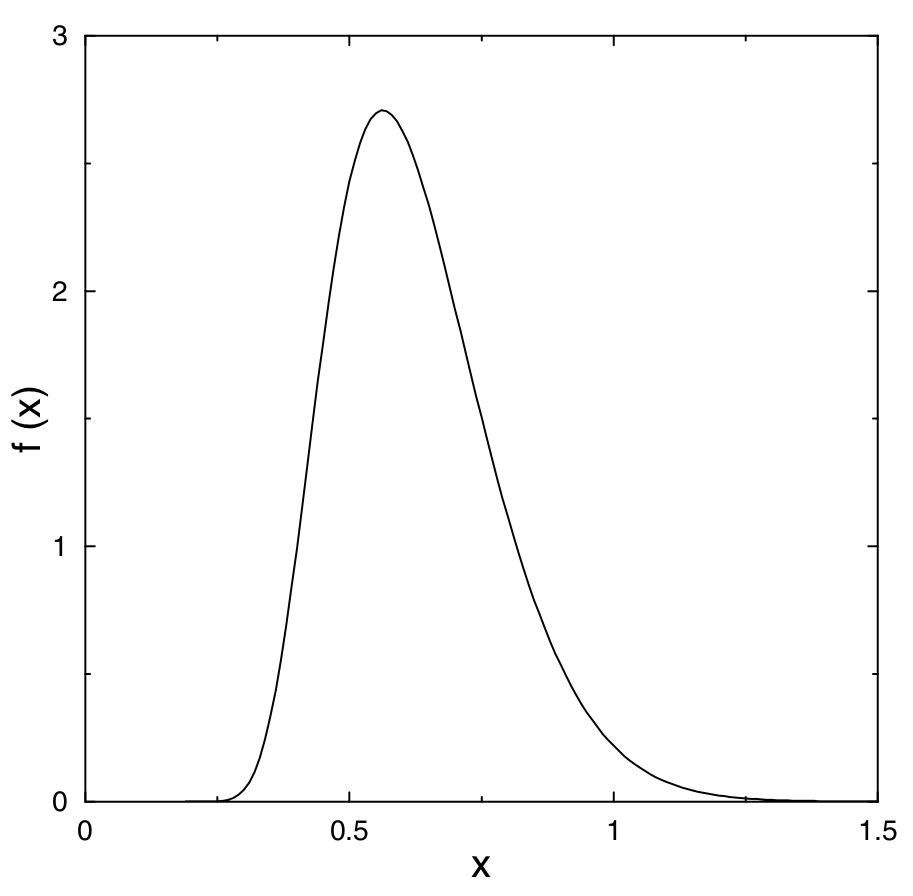
\includegraphics[width=0.5\linewidth]{intro/airyplot-majumdar.png}
    \caption{Fonction $f(x$) de la distribution des hauteurs d'une interface Edwards-Wilkinson avec des conditions aux bords périodiques\cite{majumdar_airy_2005} en 1+1 dimensions.}
     \label{fig-airy-majumdar}
\end{figure}


    \subsection{Paramètre d'ordre conservé}

Si l'on se place dans le référentiel du centre de l'interface, les équations \ref{edwards-wilkinson-conesrved} et \ref{kpz} conservent le paramètre d'ordre en moyenne. Néanmoins, la transformation $h \rightarrow h + Dt$ ne prend pas en compte les fluctuations thermiques qui viennent perturber l'interface, ce qui fait que $h(t) \neq cte$. L'astuce vient ici de \cite{kawasaki_diffusion_1966,kawasaki_correlation-function_1966}, où l'on reprend l'équation de Cahn-Hilliard-Cook pour les interfaces
\begin{align}
    \frac{\partial h}{\partial t} = D \nabla^2 \frac{\delta H}{\delta h} +  \eta(x,t)
\end{align}
qui nous donne l'équation Villain-Lai-Das Sarma\cite{villain_continuum_1991,lai_kinetic_1991}
\begin{align}
    \frac{\partial h}{\partial t} = - D \nabla^4 h + \lambda \nabla^2 (\nabla h) ^2 +  \eta(x,t)
\end{align}
qui a fait l'objet de nombreuses études\cite{kim_conserved_1994,assis_dynamic_2015}.

L'intérêt d'un tel système est qu'il est contraint à une dynamique locale qui permet d'obtenir un système hors-équilibre. La distribution de la hauteur de l'interface respecte ici aussi le régime d'échelle  \cite{oliveira_maximal-_2008,singha_renormalization_2016} dans le régime transient. 

    \section{Cisaillement d'une interface}
{\color{red} enrichir de résultats et manips}
Il suffit d'avoir une force conservative dans le système pour qu'il soit hors-équilibre, le cisaillement en est l'expression la plus simple. Le cisaillement intervient dans la sédimentation des particules, le mouvement forcé de particules chargées dans un champ électrique ou bien par la pression de radiation exercée par un laser. 
Dans un cisaillement, certaines particules ont tendance à bouger préférentiellement dans un sens par rapport aux autres particules, impliquant un flux non nul. Cette dynamique étant locale, elle ne peut exister que si le paramètre d'ordre est conservé. L'équation générale d'un système d'interface avec un cisaillement est\cite{bray_interface_2001-1,bray_interface_2001}
\begin{align}
     \frac{\partial h}{\partial t} + v \nabla h =  \mathcal{L} h +  \eta(x,t)
     \label{eq-cisaillement}
\end{align}
où l'opérateur $\mathcal{L}$ est associé au modèle A ou B, et le terme $v \nabla h$ est un terme de d'advection du au flux produit par le cisaillement. 


Le cisaillement le plus évident est un cisaillement homogène, par exemple un champ gravitationel qui sédimente les particules. Dans ce cas, le champ de vitesse $v$ étant constant, l'équation \ref{eq-cisaillement} est invariante par la transformation galiléenne $x \rightarrow x+vt$. 
Néanmoins de nombreuses expériences\cite{derks_suppression_2006} et simulations numériques \cite{leung_field_1986,rikvold_microstructure_2002,gonnella_nonequilibrium_2009,smith_driven_2010,smith_interfaces_2008,sadhu_non-local_2014,cohen_interface_2016} montrent que le cisaillement provoque un confinement de l'interface. Dans les expériences, cette invariance galiléenne est brisée par la disparité du champ de vitesse sur les différentes particules, comme expliqué en détail au chapitre \ref{chap-article-dean} \footnote{Ce chapitre a été publié dans \cite{dean_effect_2020}.}
Pour les simulations numériques, l'invariance est brisée par la dynamique même du système, puisque les mouvements sont fait séquentiellement. 
